
\documentclass[letterpaper,hide notes,xcolor={table,svgnames},pdftex,10pt]{beamer}
\def\showexamples{t}


%\usepackage[svgnames]{xcolor}

%% Demo talk
%\documentclass[letterpaper,notes=show]{beamer}

\usecolortheme{crane}
\setbeamertemplate{navigation symbols}{}

\usetheme{MyPittsburgh}
%\usetheme{Frankfurt}

%\usepackage{tipa}

\usepackage{hyperref}
\usepackage{graphicx,xspace}
\usepackage[normalem]{ulem}
\usepackage{multicol}

\newcommand\SF[1]{$\bigstar$\footnote{SF: #1}}

\usepackage[default]{sourcesanspro}
\usepackage[T1]{fontenc}

\newcounter{tmpnumSlide}
\newcounter{tmpnumNote}

% old question code
%\newcommand\question[1]{{$\bigstar$ \small \onlySlide{2}{#1}}}
% \newcommand\nquestion[1]{\ifdefined \presentationonly \textcircled{?} \fi \note{\par{\Large \textbf{?}} #1}}
% \newcommand\nanswer[1]{\note{\par{\Large \textbf{A}} #1}}


 \newcommand\mnote[1]{%
   \addtocounter{tmpnumSlide}{1}
   \ifdefined\showcues {~\tiny\fbox{\arabic{tmpnumSlide}}}\fi
   \note{\setlength{\parskip}{1ex}\addtocounter{tmpnumNote}{1}\textbf{\Large \arabic{tmpnumNote}:} {#1\par}}}

\newcommand\mmnote[1]{\note{\setlength{\parskip}{1ex}#1\par}}

%\newcommand\mnote[2][]{\ifdefined\handoutwithnotes {~\tiny\fbox{#1}}\fi
% \note{\setlength{\parskip}{1ex}\textbf{\Large #1:} #2\par}}

%\newcommand\mnote[2][]{{\tiny\fbox{#1}} \note{\setlength{\parskip}{1ex}\textbf{\Large #1:} #2\par}}

\newcommand\mquestion[2]{{~\color{red}\fbox{?}}\note{\setlength{\parskip}{1ex}\par{\Large \textbf{?}} #1} \note{\setlength{\parskip}{1ex}\par{\Large \textbf{A}} #2\par}\ifdefined \presentationonly \pause \fi}

\newcommand\blackboard[1]{%
\ifdefined   \showblackboard
  {#1}
  \else {\begin{center} \fbox{\colorbox{blue!30}{%
         \begin{minipage}{.95\linewidth}%
           \hspace{\stretch{1}} Some space intentionally left blank; done at the blackboard.%
         \end{minipage}}}\end{center}}%
         \fi%
}



%\newcommand\q{\tikz \node[thick,color=black,shape=circle]{?};}
%\newcommand\q{\ifdefined \presentationonly \textcircled{?} \fi}

\usepackage{listings}
\lstset{%
  keywordstyle=\bfseries,
  aboveskip=15pt,
  belowskip=15pt,
  captionpos=b,
  identifierstyle=\ttfamily,
  escapeinside={(*@}{@*)},
  stringstyle=\ttfamiliy,
  frame=lines,
  numbers=left, basicstyle=\scriptsize, numberstyle=\tiny, stepnumber=0, numbersep=2pt}

\usepackage{siunitx}
\newcommand\sius[1]{\num[group-separator = {,}]{#1}\si{\micro\second}}
\newcommand\sims[1]{\num[group-separator = {,}]{#1}\si{\milli\second}}
\newcommand\sins[1]{\num[group-separator = {,}]{#1}\si{\nano\second}}
\sisetup{group-separator = {,}, group-digits = true}

%% -------------------- tikz --------------------
\usepackage{tikz}
\usetikzlibrary{positioning}
\usetikzlibrary{arrows,backgrounds,automata,decorations.shapes,decorations.pathmorphing,decorations.markings,decorations.text}

\tikzstyle{place}=[circle,draw=blue!50,fill=blue!20,thick, inner sep=0pt,minimum size=6mm]
\tikzstyle{transition}=[rectangle,draw=black!50,fill=black!20,thick, inner sep=0pt,minimum size=4mm]

\tikzstyle{block}=[rectangle,draw=black, thick, inner sep=5pt]
\tikzstyle{bullet}=[circle,draw=black, fill=black, thin, inner sep=2pt]

\tikzstyle{pre}=[<-,shorten <=1pt,>=stealth',semithick]
\tikzstyle{post}=[->,shorten >=1pt,>=stealth',semithick]
\tikzstyle{bi}=[<->,shorten >=1pt,shorten <=1pt, >=stealth',semithick]

\tikzstyle{mut}=[-,>=stealth',semithick]

\tikzstyle{treereset}=[dashed,->, shorten >=1pt,>=stealth',thin]

\usepackage{ifmtarg}
\usepackage{xifthen}
\makeatletter
% new counter to now which frame it is within the sequence
\newcounter{multiframecounter}
% initialize buffer for previously used frame title
\gdef\lastframetitle{\textit{undefined}}
% new environment for a multi-frame
\newenvironment{multiframe}[1][]{%
\ifthenelse{\isempty{#1}}{%
% if no frame title was set via optional parameter,
% only increase sequence counter by 1
\addtocounter{multiframecounter}{1}%
}{%
% new frame title has been provided, thus
% reset sequence counter to 1 and buffer frame title for later use
\setcounter{multiframecounter}{1}%
\gdef\lastframetitle{#1}%
}%
% start conventional frame environment and
% automatically set frame title followed by sequence counter
\begin{frame}%
\frametitle{\lastframetitle~{\normalfont(\arabic{multiframecounter})}}%
}{%
\end{frame}%
}
\makeatother

\makeatletter
\newdimen\tu@tmpa%
\newdimen\ydiffl%
\newdimen\xdiffl%
\newcommand\ydiff[2]{%
    \coordinate (tmpnamea) at (#1);%
    \coordinate (tmpnameb) at (#2);%
    \pgfextracty{\tu@tmpa}{\pgfpointanchor{tmpnamea}{center}}%
    \pgfextracty{\ydiffl}{\pgfpointanchor{tmpnameb}{center}}%
    \advance\ydiffl by -\tu@tmpa%
}
\newcommand\xdiff[2]{%
    \coordinate (tmpnamea) at (#1);%
    \coordinate (tmpnameb) at (#2);%
    \pgfextractx{\tu@tmpa}{\pgfpointanchor{tmpnamea}{center}}%
    \pgfextractx{\xdiffl}{\pgfpointanchor{tmpnameb}{center}}%
    \advance\xdiffl by -\tu@tmpa%
}
\makeatother
\newcommand{\copyrightbox}[3][r]{%
\begin{tikzpicture}%
\node[inner sep=0pt,minimum size=2em](ciimage){#2};
\usefont{OT1}{phv}{n}{n}\fontsize{4}{4}\selectfont
\ydiff{ciimage.south}{ciimage.north}
\xdiff{ciimage.west}{ciimage.east}
\ifthenelse{\equal{#1}{r}}{%
\node[inner sep=0pt,right=1ex of ciimage.south east,anchor=north west,rotate=90]%
{\raggedleft\color{black!50}\parbox{\the\ydiffl}{\raggedright{}#3}};%
}{%
\ifthenelse{\equal{#1}{l}}{%
\node[inner sep=0pt,right=1ex of ciimage.south west,anchor=south west,rotate=90]%
{\raggedleft\color{black!50}\parbox{\the\ydiffl}{\raggedright{}#3}};%
}{%
\node[inner sep=0pt,below=1ex of ciimage.south west,anchor=north west]%
{\raggedleft\color{black!50}\parbox{\the\xdiffl}{\raggedright{}#3}};%
}
}
\end{tikzpicture}
}


%% --------------------

%\usepackage[excludeor]{everyhook}
%\PushPreHook{par}{\setbox0=\lastbox\llap{MUH}}\box0}

%\vspace*{\stretch{1}

%\setbox0=\lastbox \llap{\textbullet\enskip}\box0}

\setlength{\parskip}{\fill}

\newcommand\noskips{\setlength{\parskip}{1ex}}
\newcommand\doskips{\setlength{\parskip}{\fill}}

\newcommand\xx{\par\vspace*{\stretch{1}}\par}
\newcommand\xxs{\par\vspace*{2ex}\par}
\newcommand\tuple[1]{\langle #1 \rangle}
\newcommand\code[1]{{\sf \footnotesize #1}}
\newcommand\ex[1]{\uline{Example:} \ifdefined \presentationonly \pause \fi
  \ifdefined\showexamples#1\xspace\else{\uline{\hspace*{2cm}}}\fi}

\newcommand\ceil[1]{\lceil #1 \rceil}


\AtBeginSection[]
{
   \begin{frame}
       \frametitle{Outline}
       \tableofcontents[currentsection]
   \end{frame}
}



\pgfdeclarelayer{edgelayer}
\pgfdeclarelayer{nodelayer}
\pgfsetlayers{edgelayer,nodelayer,main}

\tikzstyle{none}=[inner sep=0pt]
\tikzstyle{rn}=[circle,fill=Red,draw=Black,line width=0.8 pt]
\tikzstyle{gn}=[circle,fill=Lime,draw=Black,line width=0.8 pt]
\tikzstyle{yn}=[circle,fill=Yellow,draw=Black,line width=0.8 pt]
\tikzstyle{empty}=[circle,fill=White,draw=Black]
\tikzstyle{bw} = [rectangle, draw, fill=blue!20, 
    text width=4em, text centered, rounded corners, minimum height=2em]
    
    \newcommand{\CcNote}[1]{% longname
	This work is licensed under the \textit{Creative Commons #1 3.0 License}.%
}
\newcommand{\CcImageBy}[1]{%
	\includegraphics[scale=#1]{creative_commons/cc_by_30.pdf}%
}
\newcommand{\CcImageSa}[1]{%
	\includegraphics[scale=#1]{creative_commons/cc_sa_30.pdf}%
}
\newcommand{\CcImageNc}[1]{%
	\includegraphics[scale=#1]{creative_commons/cc_nc_30.pdf}%
}
\newcommand{\CcGroupBySa}[2]{% zoom, gap
	\CcImageBy{#1}\hspace*{#2}\CcImageNc{#1}\hspace*{#2}\CcImageSa{#1}%
}
\newcommand{\CcLongnameByNcSa}{Attribution-NonCommercial-ShareAlike}

\newenvironment{changemargin}[1]{% 
  \begin{list}{}{% 
    \setlength{\topsep}{0pt}% 
    \setlength{\leftmargin}{#1}% 
    \setlength{\rightmargin}{1em}
    \setlength{\listparindent}{\parindent}% 
    \setlength{\itemindent}{\parindent}% 
    \setlength{\parsep}{\parskip}% 
  }% 
  \item[]}{\end{list}} 




\title{Lecture 23 --- Professional Engineers Act \& Ontario~Regulation~941 }

\author{Jeff Zarnett, based on original by Douglas Harder \\ \small \texttt{jzarnett@uwaterloo.ca} / \texttt{dwharder@uwaterloo.ca}}
\institute{Department of Electrical and Computer Engineering \\
  University of Waterloo}
\date{\today}


\begin{document}

\begin{frame}
  \titlepage

\begin{center}
  \small{Acknowledgments: Douglas Harder~\cite{dwh}, Julie Vale~\cite{jv}}
  \end{center}
\end{frame}



\begin{frame}
\frametitle{The Act}

The Professional Engineers Act is a provincial law (statute) that governs the practice of engineering.

The professional association -- Professional Engineers Ontario -- is empowered and mandated by this act to regulate the practice in Ontario.

The association was established 14 June, 1922 and consists of multiple chapters by region (e.g., ``Grand River'').

The Act, in section 2, officially recognizes PEO as the official regulator.

\end{frame}


\begin{frame}
\frametitle{Principal Object of the Association}

Section (3) of the Act says:

\begin{quote}
The principal object of the Association is to regulate the practice of professional engineering and to govern its members, holders of certificates of authorization, holders of temporary licences, holders of provisional licences and holders of limited licences in accordance with this Act, the regulations and the by-laws in order that the public interest may be served and protected. 
\end{quote}

(In this usage, ``object'' is like ``objective''.)

\end{frame}



\begin{frame}
\frametitle{Additional Objects}


For the purpose of carrying out its principal object, the Association has the following additional objects:

\begin{enumerate}

	\item To establish, maintain and develop standards of knowledge and skill among its members.

	\item To establish, maintain and develop standards of qualification and standards of practice for the practice of professional engineering.

	\item To establish, maintain and develop standards of professional ethics among its members.

	\item To promote public awareness of the role of the Association.

	\item To perform such other duties and exercise such other powers as are imposed or conferred on the Association by or under any Act. 
	
\end{enumerate}

\end{frame}



\begin{frame}
\frametitle{Overview of PEO}

\begin{center}
	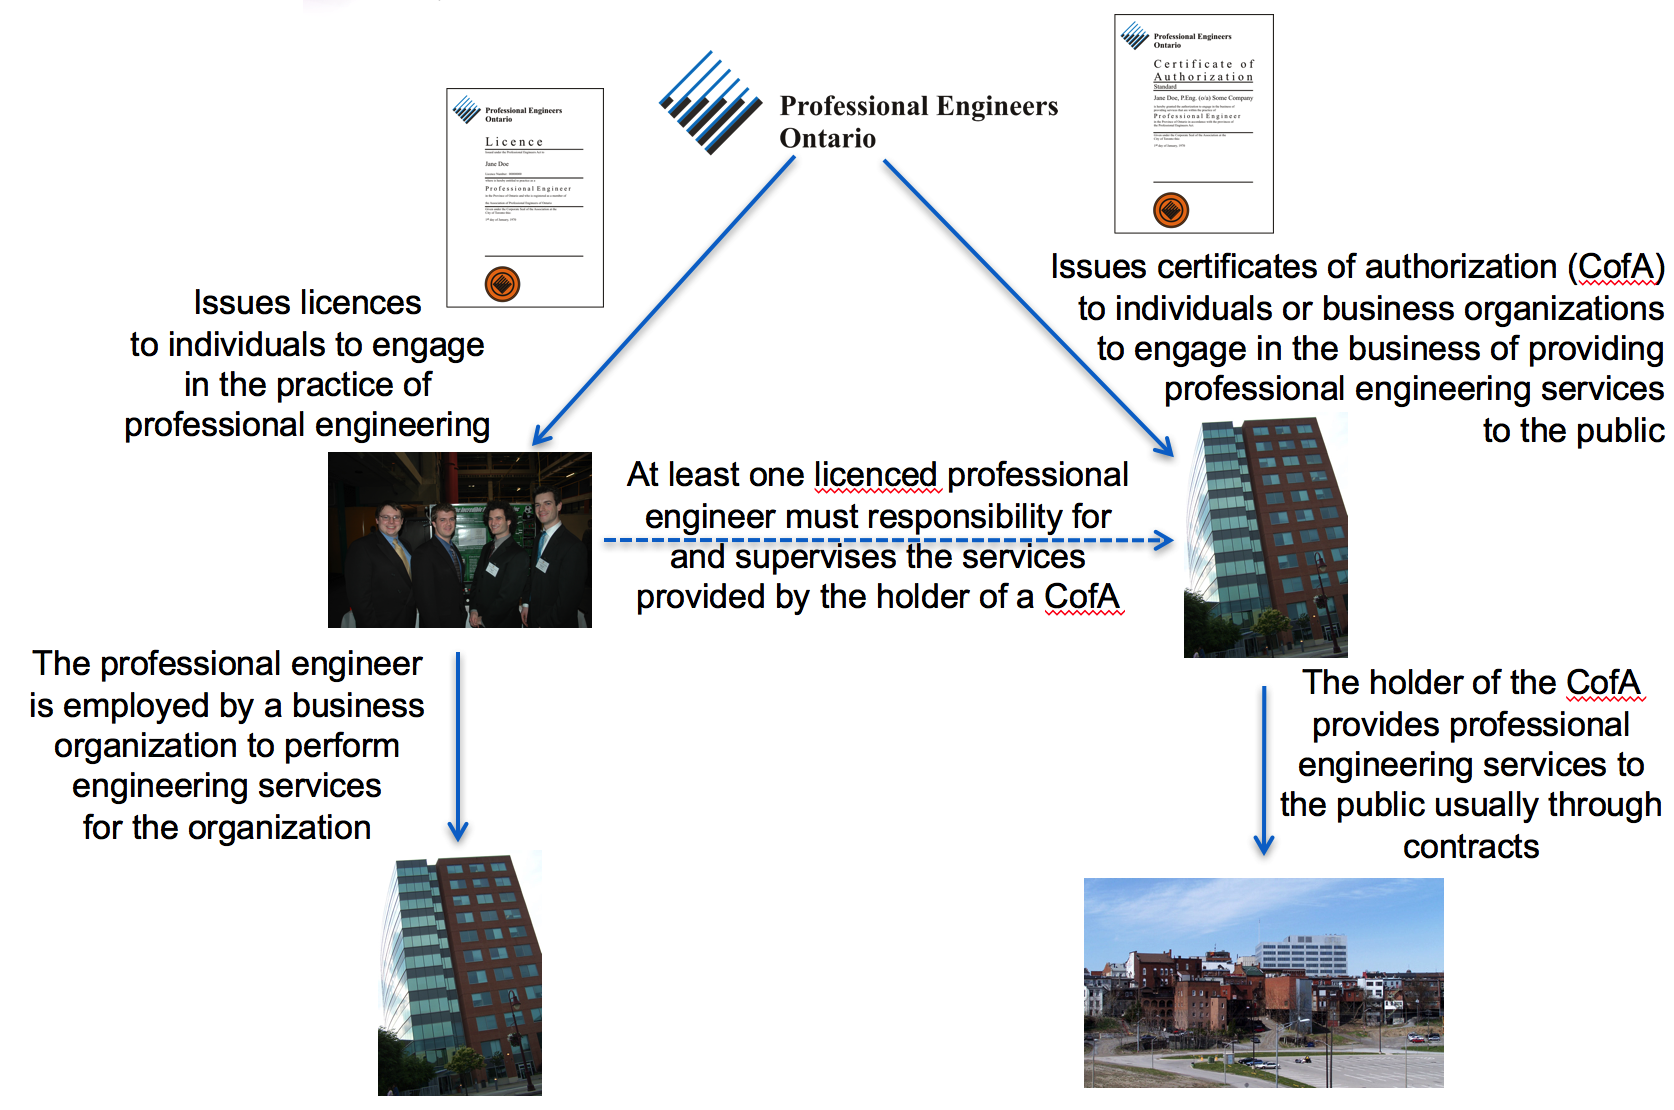
\includegraphics[width=0.9\textwidth]{images/PEO-Overview}\\
	{\scriptsize Image Credit: D. W. Harder}
\end{center}

\end{frame}



\begin{frame}
\frametitle{PEO Structure}

The act defines:

\begin{itemize}
\item The objectives of the association and its council
\item Meetings, membership, regulations, by-laws, and publications
\item The powers of the Attorney General
\item The framework for licensure and certification
\item The duties and powers of the various committees and councillors
\item The requirement for insurance
\item Details regarding discipline and enforcement
\end{itemize}

\end{frame}



\begin{frame}
\frametitle{Law vs. Regulations}

The legislative branch of parliament enacts statutes.

Only an act of parliament can compel the government to spend money.

The executive branch may enact regulations, codes, orders-in-council, etc.
PEO may make regulations through the approval of the Lieutenant Governor.

Regulations are subject to review by the Attorney General.

The Attorney General is a member of the Cabinet or Executive Council.

The Attorney General is the chief legal advisor to the government with the responsibility for the oversight of the justice system within the province.


\end{frame}



\begin{frame}
\frametitle{Why Provincial?}


The reason that this is a provincial act and not an act of the federal Parliament of Canada is that the Constitution of Canada prescribes:

\begin{quote}  
In each Province the Legislature may exclusively make Laws in
		relation to Matters coming within the Classes of Subjects next
		hereinafter enumerated; that is to say,\\
				10.	Local Works and Undertakings ...
\end{quote}

	The practice of professional engineering falls, at least, under that clause.

\end{frame}



\begin{frame}
\frametitle{How Does Regulation Work?}

Section 7(1) of the Professional Engineers Act specifies those items with respect to which PEO may make regulations.

The regulations are published under Ontario Regulation 941.

There are 34 items listed in the act (a couple of which are repealed).

There are 88 sections in O.Reg. 941.

Each of the 88 sections must in some way regulate at least one aspect of one of the items in the act.


\end{frame}


\begin{frame}
\frametitle{How Does PEO Regulate?}

PEO regulates the practice of professional engineering through:

1. Issuing of licences to those qualified to engage in the practice of professional engineering.

2. Issuing of Certificates of Authorization for to organizations wishing to do business offering professional engineering services to the public.


\end{frame}



\begin{frame}
\frametitle{Licences}

Licence, \textit{n}.
\begin{quote}
A formal, usually a printed or written permission from a constituted authority to do something, e.g. to marry, to print or publish a book, to preach, to carry on some trade, etc.; a permit.
\end{quote}

License, \textit{v},
\begin{quote}
To grant (a person) a licence or authoritative permission to hold a certain status or to do certain things, e.g. to practise some trade or profession, to hold a curacy, to preach, to use armorial bearings, to keep a dog, to carry a gun, etc.
\end{quote}

Source: Oxford English Dictionary

\end{frame}



\begin{frame}
\frametitle{Licences}

PEO issues licences to natural persons who have satisfied:

The general requirements for licensure stated in the Professional Engineers Act AND the specific requirements for licensure listed in the regulations.

\end{frame}




\begin{frame}
\frametitle{Issuance of Licence}

14.  (1)  The Registrar shall issue a licence to a natural person who applies therefor in accordance with the regulations and,
\begin{enumerate}[(a)]
\item		\sout{Repealed:  is a Canadian citizen;}\\
\item	is not less than eighteen years of age;\\
\item	has complied with the academic requirements specified in
		the regulations ..., including passing such examinations as
		the Council sets or approves ..., or is exempted by the
		Council from complying with the requirements;\\
\item	has complied with the experience requirements specified in
		the regulations for the issuance of the licence;\\
\item	has complied with any other requirements specified in the
		regulations for the issuance of the licence; and\\
\item	is of good character.
\end{enumerate}
\end{frame}




\begin{frame}
\frametitle{Relevant Regulations}

33. (1) Each applicant for a licence shall comply with the following rules:
\begin{enumerate}
\item The applicant shall demonstrate that he or she has obtained,
	\begin{enumerate}[i)]
	\item a bachelor's degree in an engineering program from a
		Canadian university that is accredited..., or
	\item equivalent engineering educational qualifications 
	\end{enumerate}
\item 48 months of experience in the practice of professional engineering that provides sufficient experience
\item Up to 12 months of the practical experience referred to in paragraph 2 may be acquired after the applicant has completed one-half of the classroom component of the degree...
\item At least 12 months of the balance shall be acquired in a Canadian jurisdiction
\item The applicant shall successfully complete the Professional
Practice Examination
\end{enumerate}

\end{frame}



\begin{frame}
\frametitle{Canadian Experience Requirement}


Experience acquired outside Canada satisfies the requirements of paragraph 4 of subsection (1) if,

\begin{enumerate}[(a)]
\item it is obtained while the applicant is,

\begin{enumerate}[i)]
\item employed by an employer whose head office is located in Canada, and

\item supervised by one or more persons who are legally authorized to engage in the practice of professional engineering in a Canadian jurisdiction; and
\end{enumerate}

\item in the Council's opinion, the experience provides the applicant with,

\begin{enumerate}[i)]
\item the necessary practical skill for the practice of professional engineering, and

\item sufficient familiarity with the applicable Canadian codes, regulations and standards for the practice of professional engineering.
\end{enumerate}

\end{enumerate}

\end{frame}



\begin{frame}
\frametitle{Restrictions on Practice}

Is a civil engineer allowed to engage in the field of electrical engineering?


Konrad Zuse, who designed the first programmable electronic computer  -- which happened to be Turing complete, was a civil engineer.

When you get your licence, you will note that there are no restrictions.

In theory, someone who studies electrical engineering can approve a building's construction. 

Is this a good idea?

\end{frame}



\begin{frame}
\frametitle{Restrictions on Practice}

Holders have a responsibility to not undertake work they are not competent to perform by virtue of their training and experience.

Doing so is professional misconduct...

\end{frame}



\begin{frame}
\frametitle{Structure of PEO}

The members of PEO are those who have licences to engage in the practice of professional engineering.

The majority of the Council are Members who are elected by Members.

Members comprise the majority of all committees:

\begin{itemize}
\item Executive Committee
\item Academic Requirements Committee
\item Experience Requirements Committee
\item Registration Committee
\item Complaints Committee
\item Discipline Committee
\item Enforcement Committee
\item Fees Mediation Committee
\end{itemize}

As well as other committees...

\end{frame}



\begin{frame}
\frametitle{Other Licenses}

The all-or-nothing approach that requires everyone who engages in the practice to have a license, or be supervised by someone with one, is a little strict.

Consider the following scenarios:

What if a professional engineer from another jurisdiction needs to be brought in for one specialized project?

What if a professional engineer from another country has immigrated to Ontario, has all the requisite experience except experience in Canada?

\end{frame}




\begin{frame}
\frametitle{Other Licenses}

What if an individual has specialized knowledge but does not have a complete engineering degree?

What if a certified engineering technician would like to offer engineering services as a technician to the public?

Should there be other forms of license for these situations? Why (not)?

\end{frame}




\begin{frame}
\frametitle{Temporary Licenses}

Temporary licenses do exist and they require the payment of a fee and one of:

\begin{enumerate}
\item Residence in a province or territory of Canada other than Ontario and membership in an association of professional engineers in another province or territory of Canada that has objects similar to the objects of the Association and that requires qualifications for membership at least equal to the qualifications required for the issuance of a licence to engage in the practice of professional engineering in Ontario.
\item Qualifications at least equal to the qualifications required for the issuance of a licence to engage in the practice of professional engineering in Ontario.
\item Wide recognition in the field of the practice of professional engineering in respect of which the work to be undertaken under the temporary licence relates and not less than ten years experience in such field. 
\end{enumerate}

\end{frame}



\begin{frame}
\frametitle{Temporary Licenses}

\begin{enumerate}
	\item Every temporary licence must specify,
	\begin{enumerate}[(a)]
\item the works, facilities, machinery, equipment or other property in Ontario to which the temporary licence relates;
\item the name of the person, firm or corporation by whom the holder of the temporary licence is employed or engaged to perform services in Ontario within the practice of professional engineering;
\item the name of the Member, if any, with whom collaboration is required under this Regulation; and
\item the period of time, not exceeding twelve months, for which the temporary licence has been issued.
\end{enumerate}
	\item It is a condition of every temporary licence that the services within the practice of professional engineering that may be provided by the holder of the temporary licence are limited to the services specified in the temporary licence. 
\end{enumerate}

\end{frame}



\begin{frame}
\frametitle{Provisional Licenses}

Provisional licenses may be granted to those who have adequate engineering experience but lack the 12 months of it being in Canada. 

It comes with two conditions:

\begin{enumerate}
	\item It is valid for 12 months and may be renewed maximum once.
	\item The holder of the provisional license must be supervised by a professional engineer.
\end{enumerate}

See O.Reg. 941, section 44.1.

\end{frame}



\begin{frame}
\frametitle{Limited License}

The requirements for a limited license are:

1. One or more of the following:
\begin{enumerate}[i)]
\item A three-year diploma in engineering technology or a Bachelor of Technology degree in engineering technology from an institution approved by the Council.
\item A four-year honours science degree in a discipline and from a university approved by the Council.
\item Academic qualifications accepted by the Council as equivalent to a diploma or degree mentioned in subparagraph i or ii.
\end{enumerate}

\end{frame}

\begin{frame}
\frametitle{Limited License}

The requirements for a limited license are:

2. Thirteen years of experience in engineering work acceptable to the Council, including the years spent in obtaining the post-secondary academic training referred to in paragraph 1 with at least one year of such experience under the supervision and direction of a Member or Members or under the supervision of a person authorized to practice professional engineering in the province or territory in Canada in which the experience was acquired and at least the last two years of the experience in the services within the practice of professional engineering with respect to which the limited licence is to apply.


... as well as payment of the fee, passing the professional practice examination, and good character.

\end{frame}



\begin{frame}
\frametitle{Technology and Technologists}


In technical fields associated with professions, should technicians and technologists be allowed to practice independently?

Should dental hygienists be allowed to provide teeth-cleaning services independent of being employed by a dentist?

Should paralegals be allowed to provide legal services for lower level courts and administrative tribunals?

Should pharmacy technicians be allowed independent practice under certain restrictions?

\end{frame}



\begin{frame}
\frametitle{Certified Engineering Technologists}


There is already a class of certified engineering technicians and technologists who may practice
the application of engineering

12. (1) The work performed by a certified technician, a certified engineering technician, applied science technologist or a certified engineering technologist consists of providing technical services,
\begin{enumerate}[(a)]
\item within the framework of practices, codes and standards that are established or enforced under an Act of Ontario or of Canada
\item within the framework of published standards in the applicable industry or field; and 
\item under the technical direction of a licensed member of an appropriate profession ...
\end{enumerate}

\end{frame}



\begin{frame}
\frametitle{Certified Engineering Technologists}

CETs, however, must be associated with the holder of a Certificate of Authorization if they wish to offer services to the public.

The most recent changes to the Profession Engineers Act allow for an engineering technologist class of limited licence.

With a LET, an individual can acquire a Certificate of Authorization and provide technical services to the public.


\end{frame}



\begin{frame}
\frametitle{The C of A}

A licence identifies an individual as being qualified to engage in the practice of professional engineering.

Such an individual can be hired through an employment contract to provide professional engineering services to the employer.

Such contracts are subject to the Employment Standards Act.

What happens if a legal person is not in a position to hire a professional engineer as an employee?

\end{frame}



\begin{frame}
\frametitle{The C of A}

Recall, from the definition of a profession:\\
\quad ... prepared to exercise that skill in the interests of \textit{the public}.

For an engineer, the public is anyone other than the engineer him or herself or the engineer's employer.

An engineer who provides services to the public is said to be in \alert{independent~practice}.

Such an engineer is said to be \alert{retained} by the client.

\end{frame}



\begin{frame}
\frametitle{Employment vs Independent Practice}

{\small
\begin{tabularx}{.95\textwidth}{X|X}
	\textbf{Employment} & \textbf{Independent Practice}\\ \hline
	You work exclusively for one business entity & You are free to provide your services to more than one business entity \\ \hline
	Your employment contract addresses non-disclosure, ability to control work hours and time off, expectations related to performance, notice, termination and remuneration & Your relationships are independent contracts or relationships, or business entities purchase your time from an agency \\ \hline
	Expenses are reimbursed & You invoice your expenses \\ \hline
	You are paid a salary or wage & You are not paid if services are not performed \\ \hline
	You are provided an office and equipment on business premises & You acquire your own business facilities \\ \hline
	You have set work hours & You are not restricted as to the hours of work \\ \hline
	You are provided benefits, e.g., vacation pay & You receive no vacation pay or bonuses \\ \hline
	Your work is covered under the business entity's professional liability insurance policy & You require your own professional liability insurance\\
\end{tabularx}
}

{\scriptsize Source: \url{http://www.peo.on.ca/offering/CofA\%20_Infoguide.pdf}}

\end{frame}



\begin{frame}
\frametitle{The C of A}

The concept of certifying the offering of professional engineering services to the public is currently limited to Ontario.


In other provinces, having a licence implies you may offer your services to the public.

	The need for certification will become more clear once we look at the requirements associated with certificates of authorization.

\end{frame}



\begin{frame}
\frametitle{The Certificate of Authorization}

From the PEA, section 15:

The Registrar shall issue a certificate of authorization to a 	natural person, a partnership or a corporation that applies 	therefor in accordance with the regulations if the requirements 	and qualifications for the issuance of the certificate of 	authorization set out in the regulations are met. 

\end{frame}



\begin{frame}
\frametitle{Supervision in the CoA}

From the PEA, section 17:

It is a condition of every certificate of authorization that the 	holder of the certificate shall provide services that are within 	the practice of professional engineering only under the 	personal supervision and direction of a holder of a licence, 	temporary licence or limited licence.


\end{frame}




\begin{frame}
\frametitle{From the Regulations}

The requirements and qualifications for the issuance of a 	certificate of authorization are:

\begin{enumerate}
\item The applicant must designate one or more holders of a licence, temporary licence or limited licence, each of whom has at least five years of professional engineering experience following the conferral of a degree ... or the completion of an equivalent engineering education.
\item The application for the certificate of authorization must state that the persons named in paragraph 1 are,
\begin{enumerate}[i)]
	\item the applicant for the certificate of authorization,
	\item employees of the applicant,
	\item partners in the applicant, or
	\item employees of partners in the applicant,
\end{enumerate}
	and will devote sufficient time to the work of the applicant to carry out the responsibilities set out in paragraph 1.
\end{enumerate}

\end{frame}



\begin{frame}
\frametitle{Certificate of Authorization}

There is also a requirement of:

\begin{itemize}
	\item Liability insurance.
	\item Mandatory disclosure of not having liability insurance.
	\item Exemption from liability insurance due to one of the few exceptions (aviation hazards, shipping hazards, nuclear hazards...).
\end{itemize}


\end{frame}



\begin{frame}
\frametitle{Certificate of Authorization}

The requirements are then, condensed:
\begin{itemize}
	\item Accountability
	\item Commitment
	\item Insurance
\end{itemize}

\end{frame}




\begin{frame}
\frametitle{Signed, Sealed, and Delivered}

When a professional engineer provides a service to a member of the public, the engineer applies his or her seal onto the document.


53.	Every holder of a licence, temporary licence, provisional licence or 	limited licence who provides to the public a service that is within 	the practice of professional engineering shall sign, date and affix the 	holder's seal to every final drawing, specification, plan, report or other 	document prepared or checked by the holder as part of the service 	before it is issued. 


\end{frame}



\begin{frame}
\frametitle{Engineer's Seal}

It is a sign of: authorship, responsibility, and reliance.

\begin{center}
	
\includegraphics[width=0.3\textwidth]{images/engineer-seal}
\end{center}

\end{frame}



\begin{frame}
\frametitle{Use of the Seal}

When sealing documents:

\begin{itemize}
\item The original document must remain unsealed and it must be kept by the engineer.
\item Only duplicates of final documents should be sealed and disseminated.
\item If a preliminary or draft document must be sealed for registration purposes, the document must clearly show that it is not to be relied upon; e.g., the word ``DRAFT'' appearing both as a watermark and in bold close to the seal.
\item Electronic documents should contain an 
electronic copy of the seal and the electronic
document must be signed using a digital signature.
\end{itemize}

\end{frame}



\begin{frame}
\frametitle{Consulting Engineers}

It is significantly more work to work in independent practice than it is to work for an employer.

Independent practice requires significantly more varied skills and organization and often such skills can only be honed with practice.

How can a professional engineer identify him or herself as being experienced in independent practice?

\end{frame}



\begin{frame}
\frametitle{Consulting Engineers}

The Act makes provisions for the designation of consulting engineer.

\begin{enumerate}
\item The Council shall designate as a consulting engineer every applicant for the designation who,
\begin{enumerate}[(a)]
\item is a Member;
\item is currently engaged, and has been continuously engaged, for not less than two years or such lesser period as may be approved by the Council, in the independent practice of professional engineering in Canada;
\item has, since becoming a Member, had five or more years of professional engineering experience that is satisfactory to the Council;
\item has passed the examinations prescribed by the Council or has been exempted therefrom, pursuant to subsection (2).
\end{enumerate}
\item The Council may exempt an applicant from any of the examinations mentioned in clause (1) (d) where the Council is of the opinion that the applicant has appropriate qualifications.
\end{enumerate}

\end{frame}



\begin{frame}
\frametitle{Wrapping Up}

Throughout this course, these definitions will be used:

	A \alert{member} is a professional engineer and member of the Association of Professional Engineers Ontario (PEO).

	A \alert{practitioner} is any Member, any holder of either a Certificate of Authorization or a temporary, provisional or limited licence.

	A \alert{holder of a licence} is any Member or any holder a temporary, provisional or limited licence.

	PEA: \url{https://www.ontario.ca/laws/statute/90p28}
	
	O.Reg.941: \url{https://www.ontario.ca/laws/regulation/900941}

\end{frame}

\begin{frame}
\frametitle{References \& Disclaimer}
\bibliographystyle{alphaurl}
\setbeamertemplate{bibliography item}{\insertbiblabel}
{\scriptsize
\bibliography{290}
}
\vfill

{\tiny Disclaimer: the material presented in these lectures slides is intended for use in the course ECE~290 at the University of Waterloo and should not be relied upon as legal advice. Any reliance on these course slides by any party for any other purpose are the responsibility of such parties.  The author(s) accept(s) no responsibility for damages, if any, suffered by any party as a result of decisions made or actions based on these course slides for any other purpose than that for which it was intended.\par}


\end{frame}



\end{document}

